\chapter{CEMicro Architecture and Technology Stack}
\label{sec:arch}

How was the "is" sutation when starting?

How should it look like?

How do I get there?


\section{The existing appliction}

The existing application which this department of Capgemini is working on in a point of sales (POS) software. It is essentially the toolkit a salesman uses to create an offer for a potential customer. Since cars are a highly configurable product the POS software has to support a huge variety of options, made even more complex by the different types of cars, different types of brands, or sub-brands, and the fact that it is used across several markets and languages. Each market has its very own requirements and also their levels of hierarchy which have to be reflected within the application in terms of user management and access levels.

The part of the application which involved my task is the creation of the final offer as a printable PDF document. Depending on the object of the sale, the type of car, the current market and a host of other factors the application will decide which document template to use and will collect the appropriate lines of text and values from the database to assemble into a finished document which is then generated in the PDF format. Additionally, there are several configuration pages in the admin area of the application where these templates can be managed and the contents defined. Figure \ref{fig:pos} shows a glimpse of the rather unwieldy admin interface for the part of the document creation.

There are currently six teams of about eight developers each working on the POS application.

\begin{figure}
  \centering
  \begin{subfigure}[b]{0.5\linewidth}
    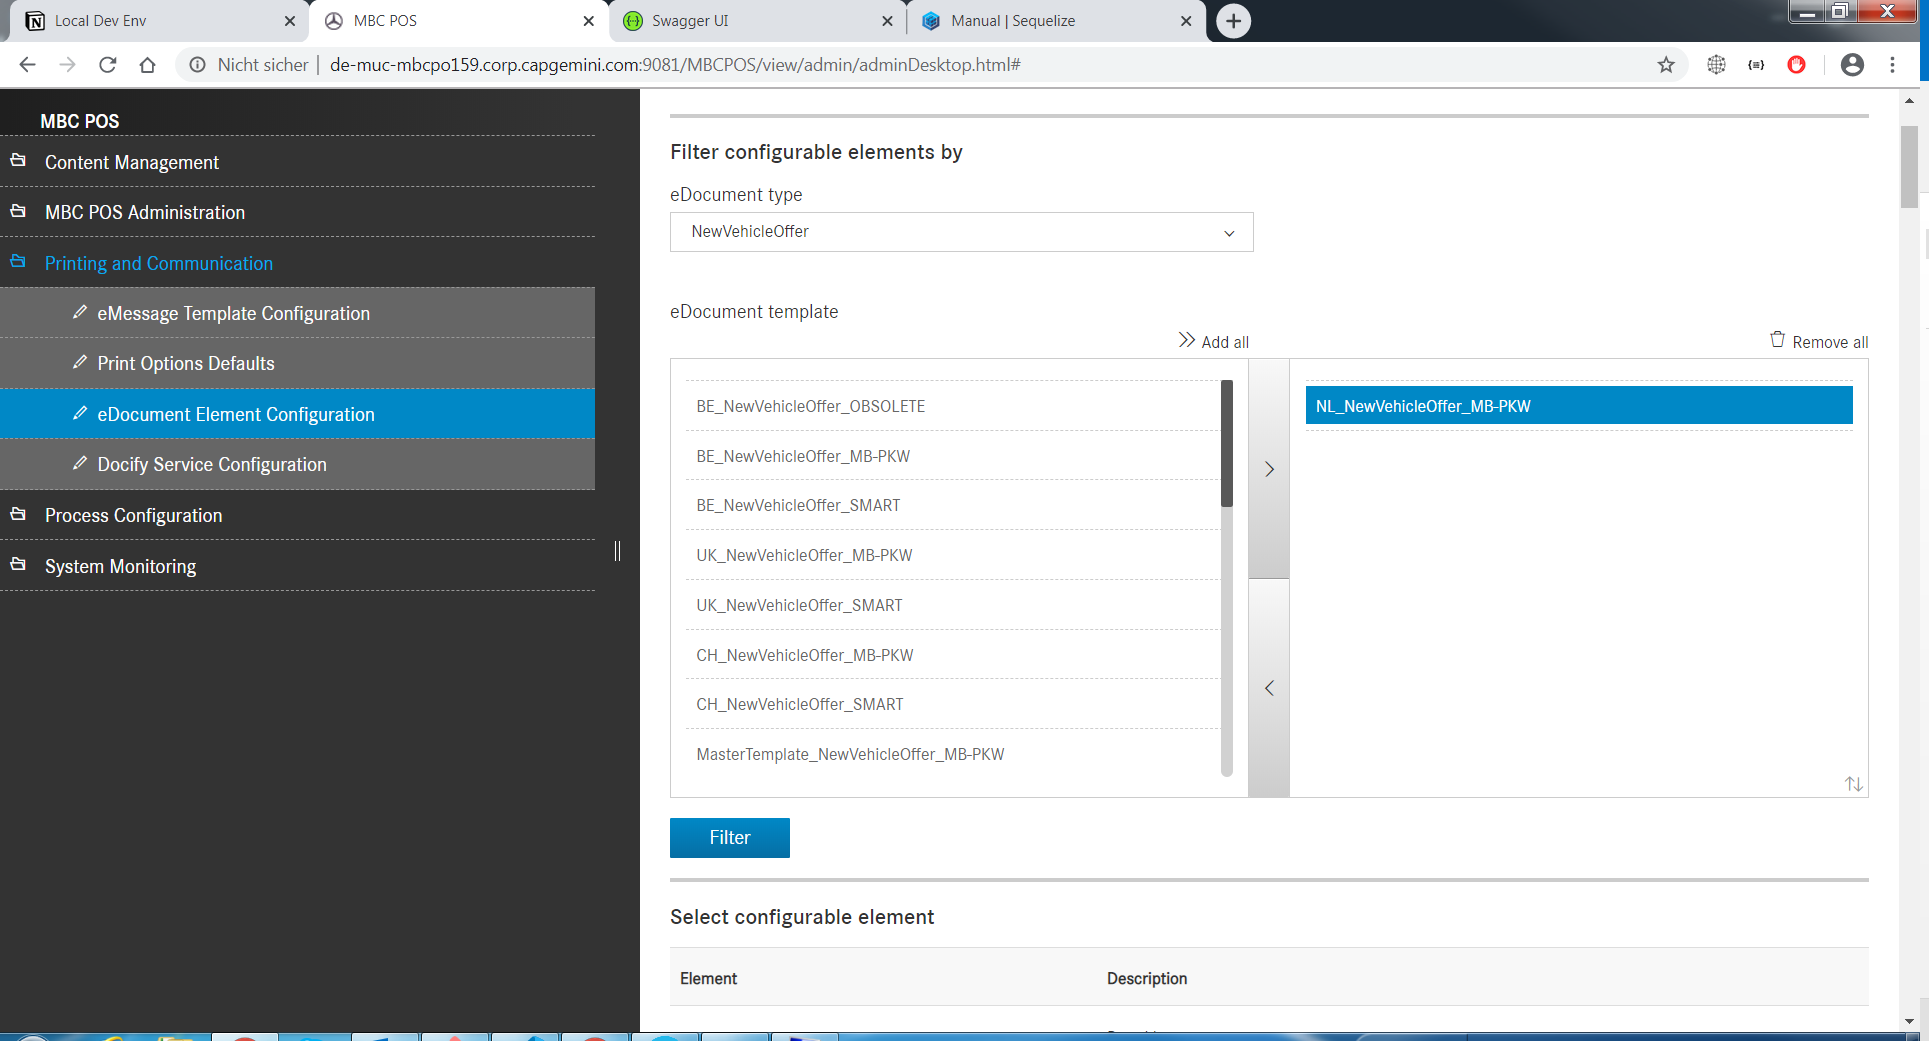
\includegraphics[width=\linewidth]{assets/pos-ce-config-1.png}
    \caption{Template selection}
  \end{subfigure}
  \begin{subfigure}[b]{0.5\linewidth}
    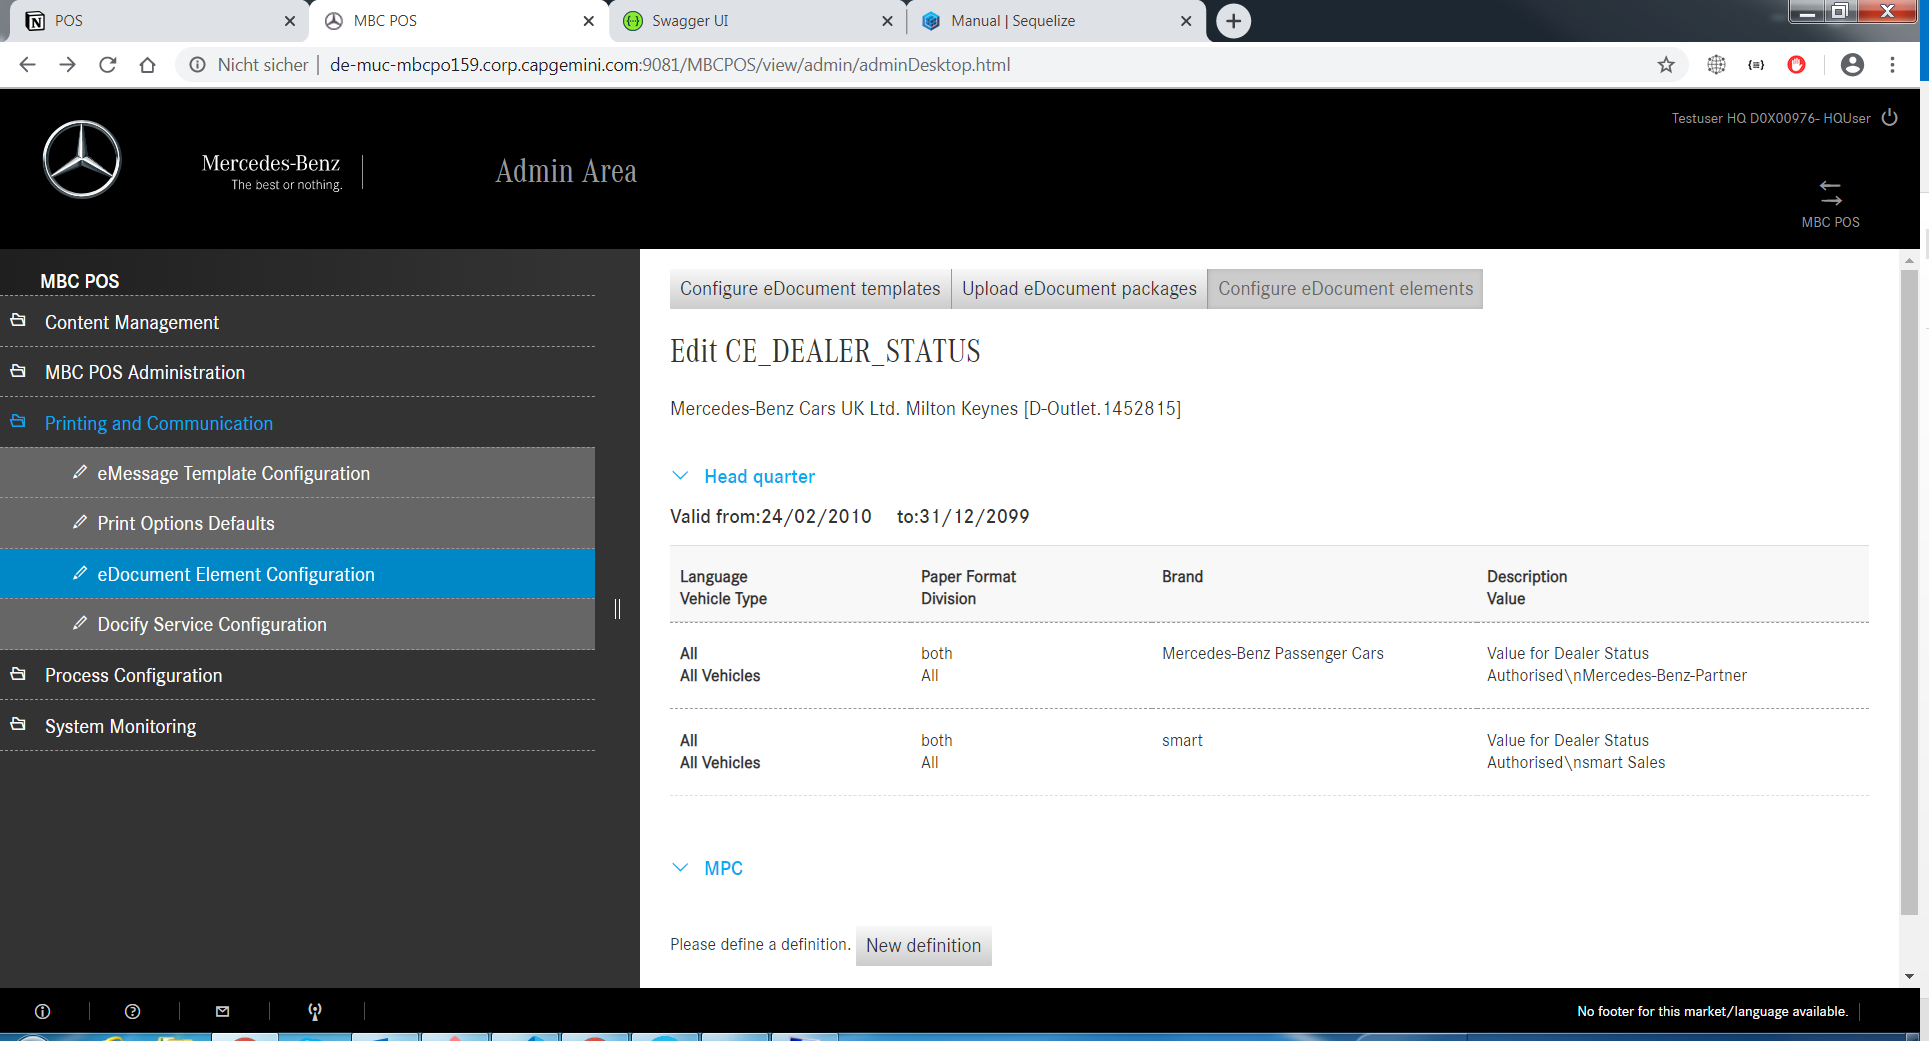
\includegraphics[width=\linewidth]{assets/pos-ce-config-3.png}
    \caption{One CE contains several children}
  \end{subfigure}
  \caption{POS configurable element admin page}
  \label{fig:pos}
\end{figure}

The part of the application responsible for generating a printable document has been part of a past student project very similar to my task. The team of students built essentially a microservice that is responsible for managing the templates and which can be called through an application programming interface (API) which returns the finished PDF. This service was named Docify.

Docify is a kind of textbook example for a microservice. A document printing service lends itself very nicely to be extracted into its separate application because its interface is so clearly defined. The interface for a printing service requires two properties, first, the name or identifier of the predefined template and second, the dataset which is needed to fill the gaps of the template. That means often the biggest challenge for distributed services, defining the boundaries and thus their interfaces are no-brainers for this use-case.

Figure \ref{fig:docify} shows the administration interface for Docify and it is easy to see how each of the two previously mentioned API criteria has their page. On the left (a) is the list of template identifiers, each template is identified by a client-market-name tuple, and on the right (b) is the editor for template specific templates with the HTML representation on the left and the rendered preview. The HTML code contains several placeholders which will be replaced by their respective value when the document is printed out.

\begin{figure}
  \centering
  \begin{subfigure}[b]{0.5\linewidth}
    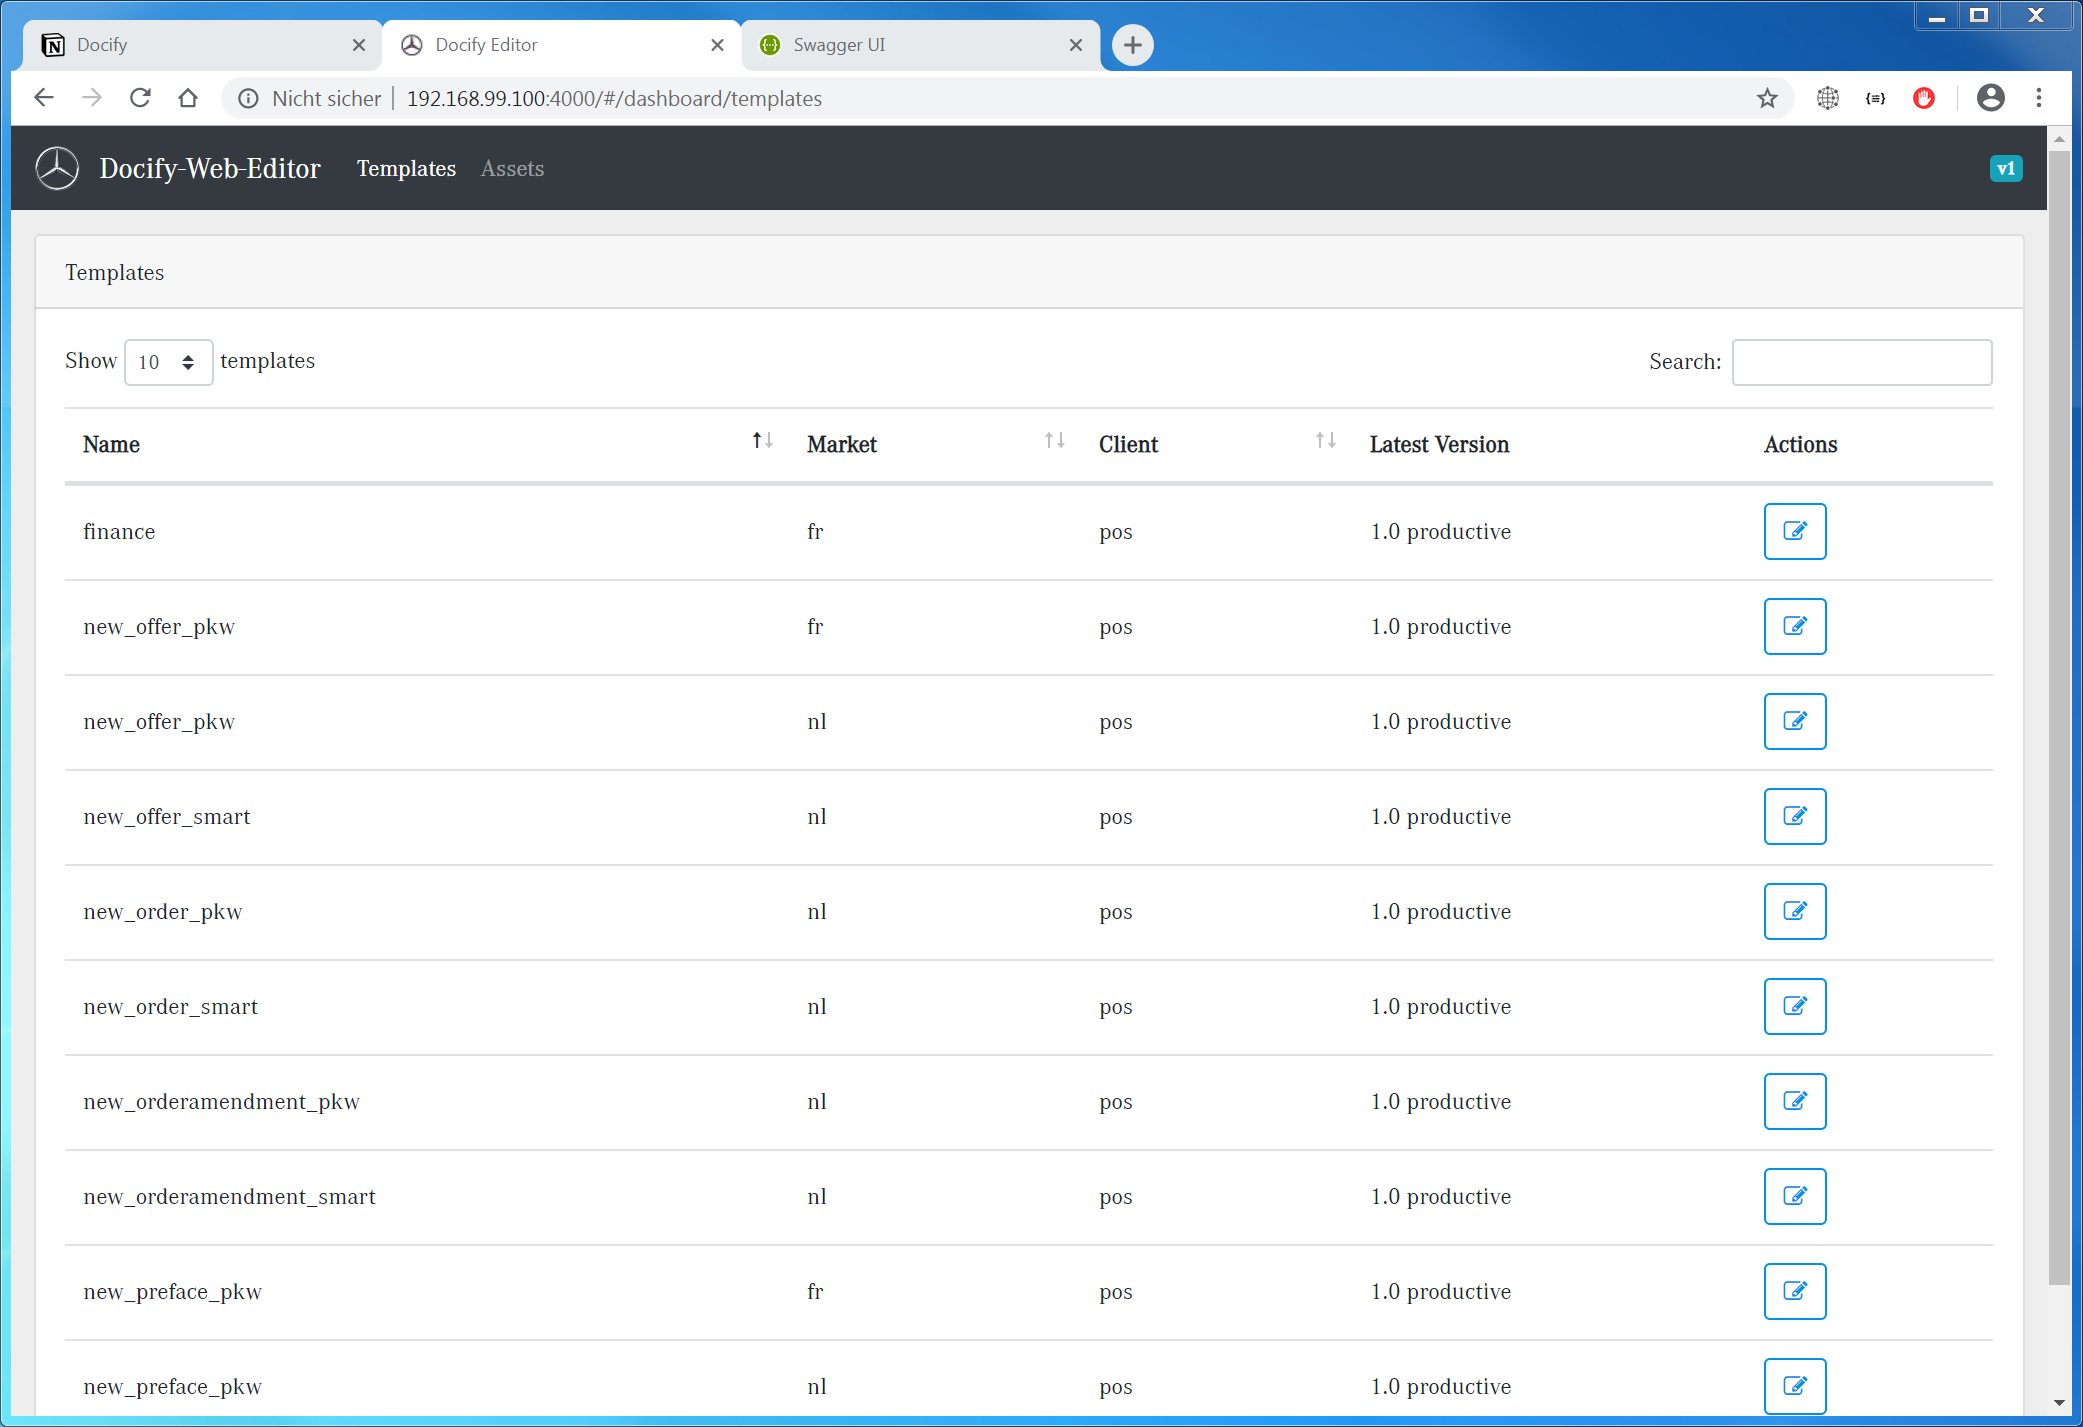
\includegraphics[width=\linewidth]{assets/docify-template-list.png}
    \caption{Template list}
  \end{subfigure}
  \begin{subfigure}[b]{0.5\linewidth}
    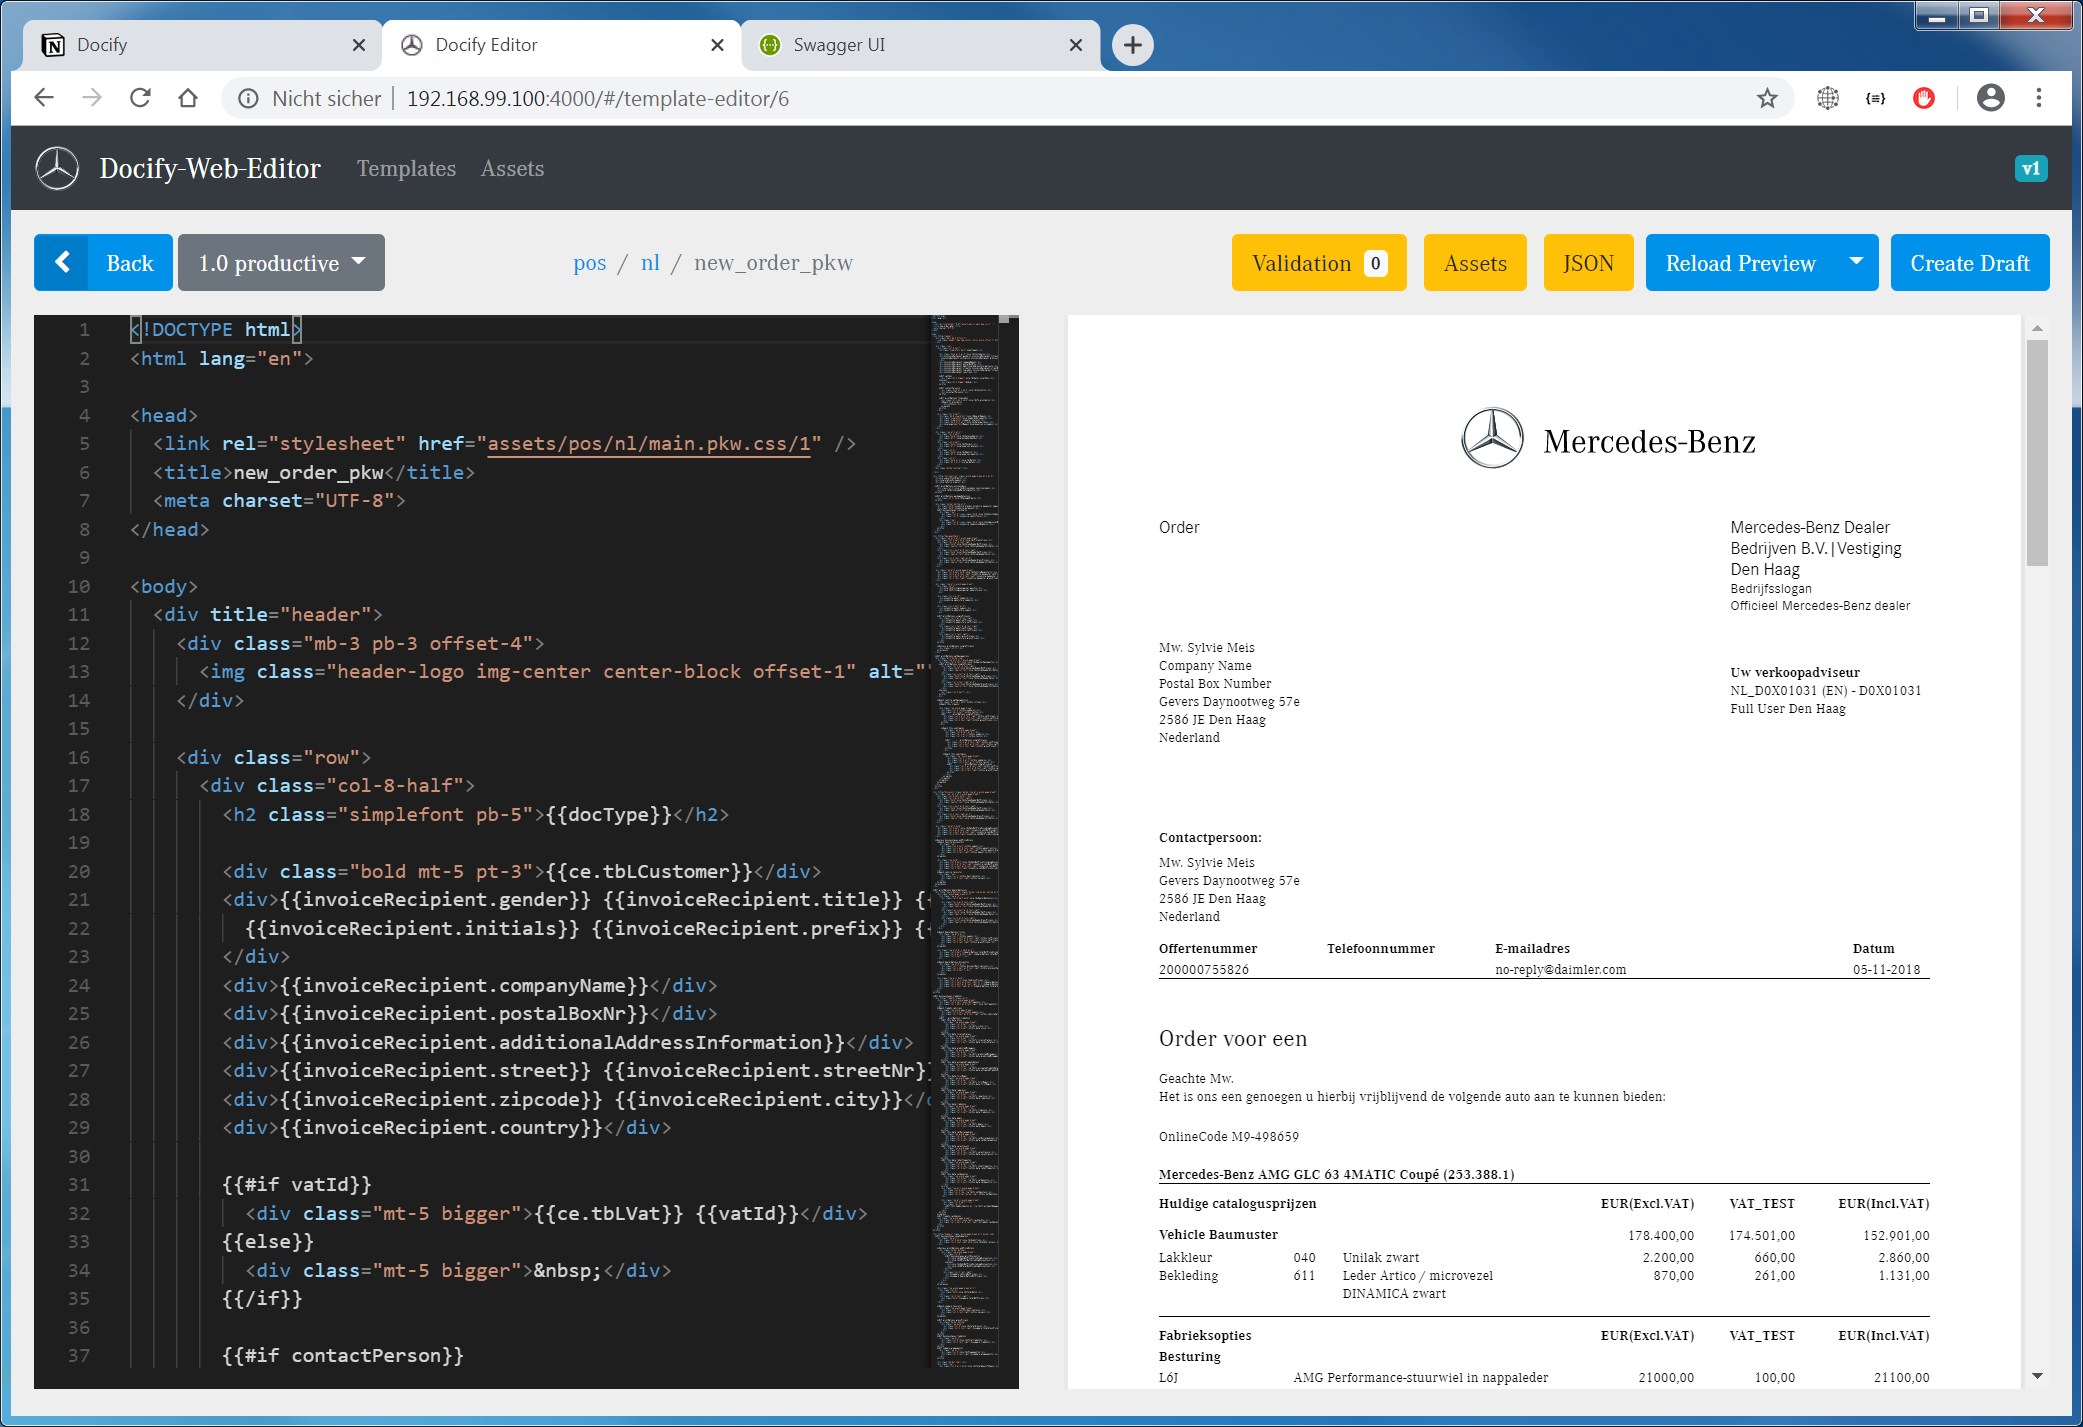
\includegraphics[width=\linewidth]{assets/docify-editor.png}
    \caption{Template editor}
  \end{subfigure}
  \caption{Docify template editor app}
  \label{fig:docify}
\end{figure}

While the technical aspect of Docify might be simple it is interesting to observe the non-technical challenges that a microservice is facing. Besides the question of how a microservice should be extracted and build there is the economic question of why it is necessary to invest the time into building such a service when it seems to be working just fine as it is. The question every project has to face is "Does it add business value?", and if it doesn't, why should the business spend money on the project? This is an interesting question especially for engineers who often try to build the ideal solution for a problem, after all, that's why we became engineers in the first place, but forget that our time is valuable and to build the ideal solution, in this case, a microservice, for an already working feature may not make much sense to the business as a whole.

So why was Docify build in the first place? I haven't been involved myself but from the proceedings with my project, I can surmise some good indicators. On the one hand, the POS application is over five years old, which in the world of software is a man with a cane and a white beard. Over the lifetime of an application, it tends to become ever more complex and both in its technical scope but also in terms of management. Thus even small changes to the codebase can take several days or even weeks until the task gets prioritized, implemented and deployed. In the ideal situation, the database contains all the parts which users are supposed to be able to edit so that changes don't have to be handed to developers, but in the case of POS, many adjustments to the document creation could only be done by direct manipulation of the codebase which meant that a task hat to be created for developers.

One example of this directly involves my task, the so-called "Configurable Elements" which I will describe in more detail in the next section are essentially texts that can be edited by users. But the definition for these elements is hardcoded in the application, meaning if users want to add a new such element they have to create a task for devs to do so, which adds considerable friction to a task which should be just one click. Essentially, Docify enables users to do administrative tasks directly while saving all the development time of adding these admin interface features to the existing monolith codebase.

The other business value has to do with the fact that there is currently a certain hype around microservice architectures. The project of Docify enabled Capgemini to showcase this architectural model on a fairly simple use-case to its client while not losing much in terms of wasted development time if the client declines its further development. And since a microservice can be built in a completely separate tech stack is was essentially a proof of concept/demo of a flashy new architecture and some flashy new technology.

In the end, the client liked what business value Docify had to offer and was willing to invest in its development. At the time of this writing, Docify is two years old and was rolled out to two of the several markets POS is operating in. Meaning even after two years of development the POS team is still maintaining the old implementation in spite of the new and shiny microservice which is probably a good image of how large companies tend to operate if their internal structures became sufficiently complex.

\section{Goals of the CEMicro Service}

What is the microservice supposed to do

High Level Overview Illustration

Complexity of POS / CE Properties

Out of scope: Access control

\begin{figure}
  \centering
  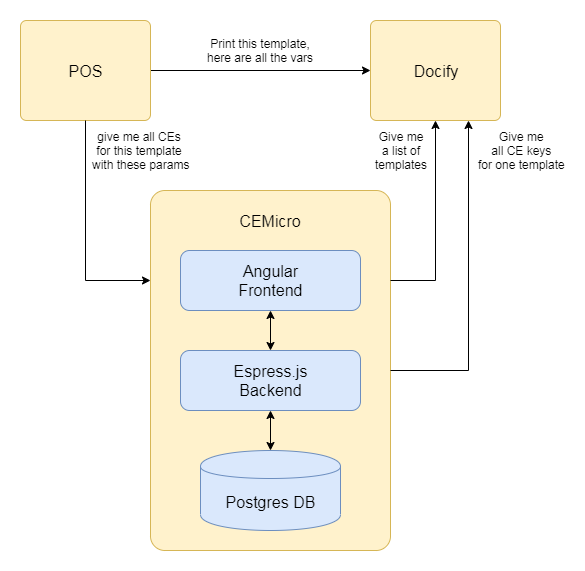
\includegraphics[width=0.6\linewidth]{assets/high-level-overview.png}
  \caption{High level context overview for the microservice}
  \label{fig:context}
\end{figure}


\section{Understanding the task}
\label{sec:arch:}

Challenge: Understanding the task

What is a configurable element?

What properties does a CE have?

Challange/Example: Devs didn't know that CEs are not uniqe per template

\begin{figure}
  \centering
  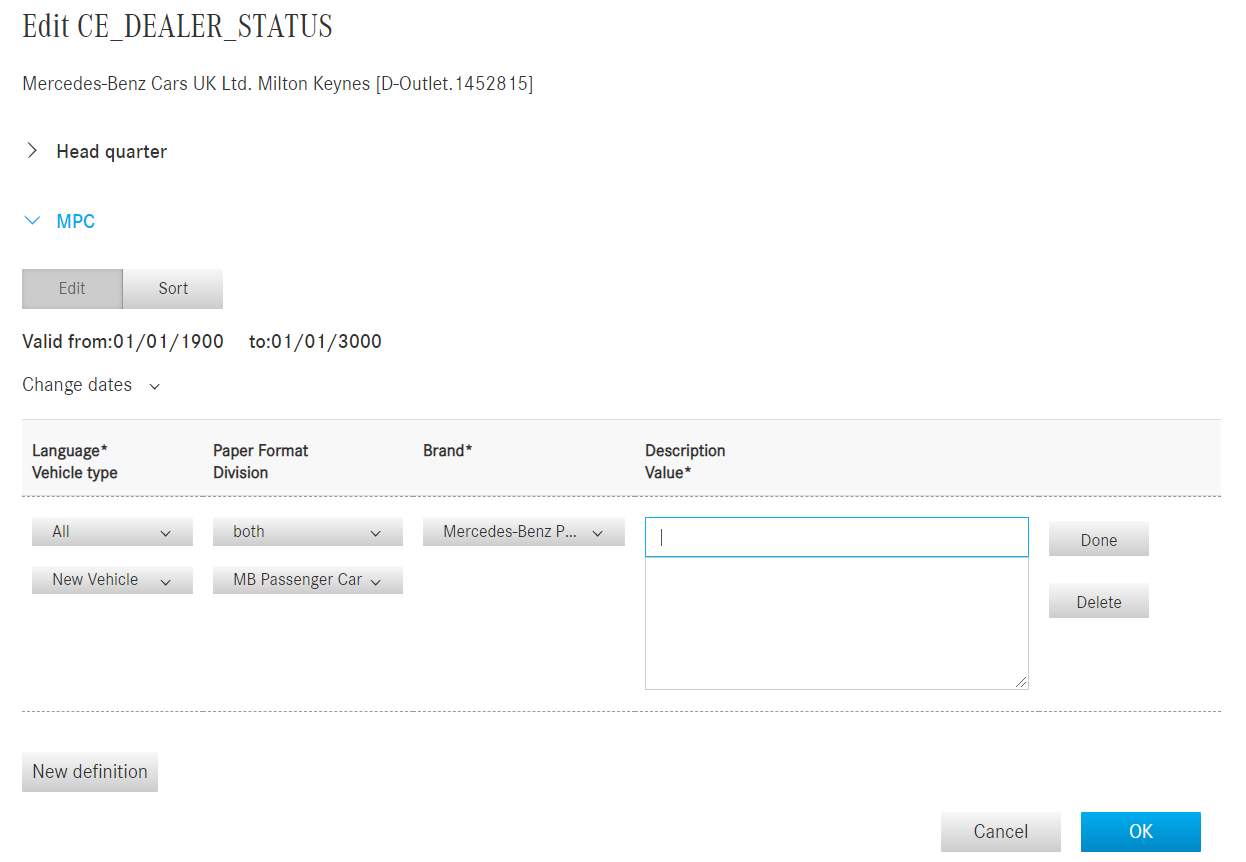
\includegraphics[width=0.8\linewidth]{assets/pos-ce-config-4.png}
  \caption{Configurable Element configuration properties}
  \label{fig:ce-properties}
\end{figure}


\section{Making optimisations}

How can the complexity of CEs be exposed in a simpler way?

\begin{figure}
  \centering
  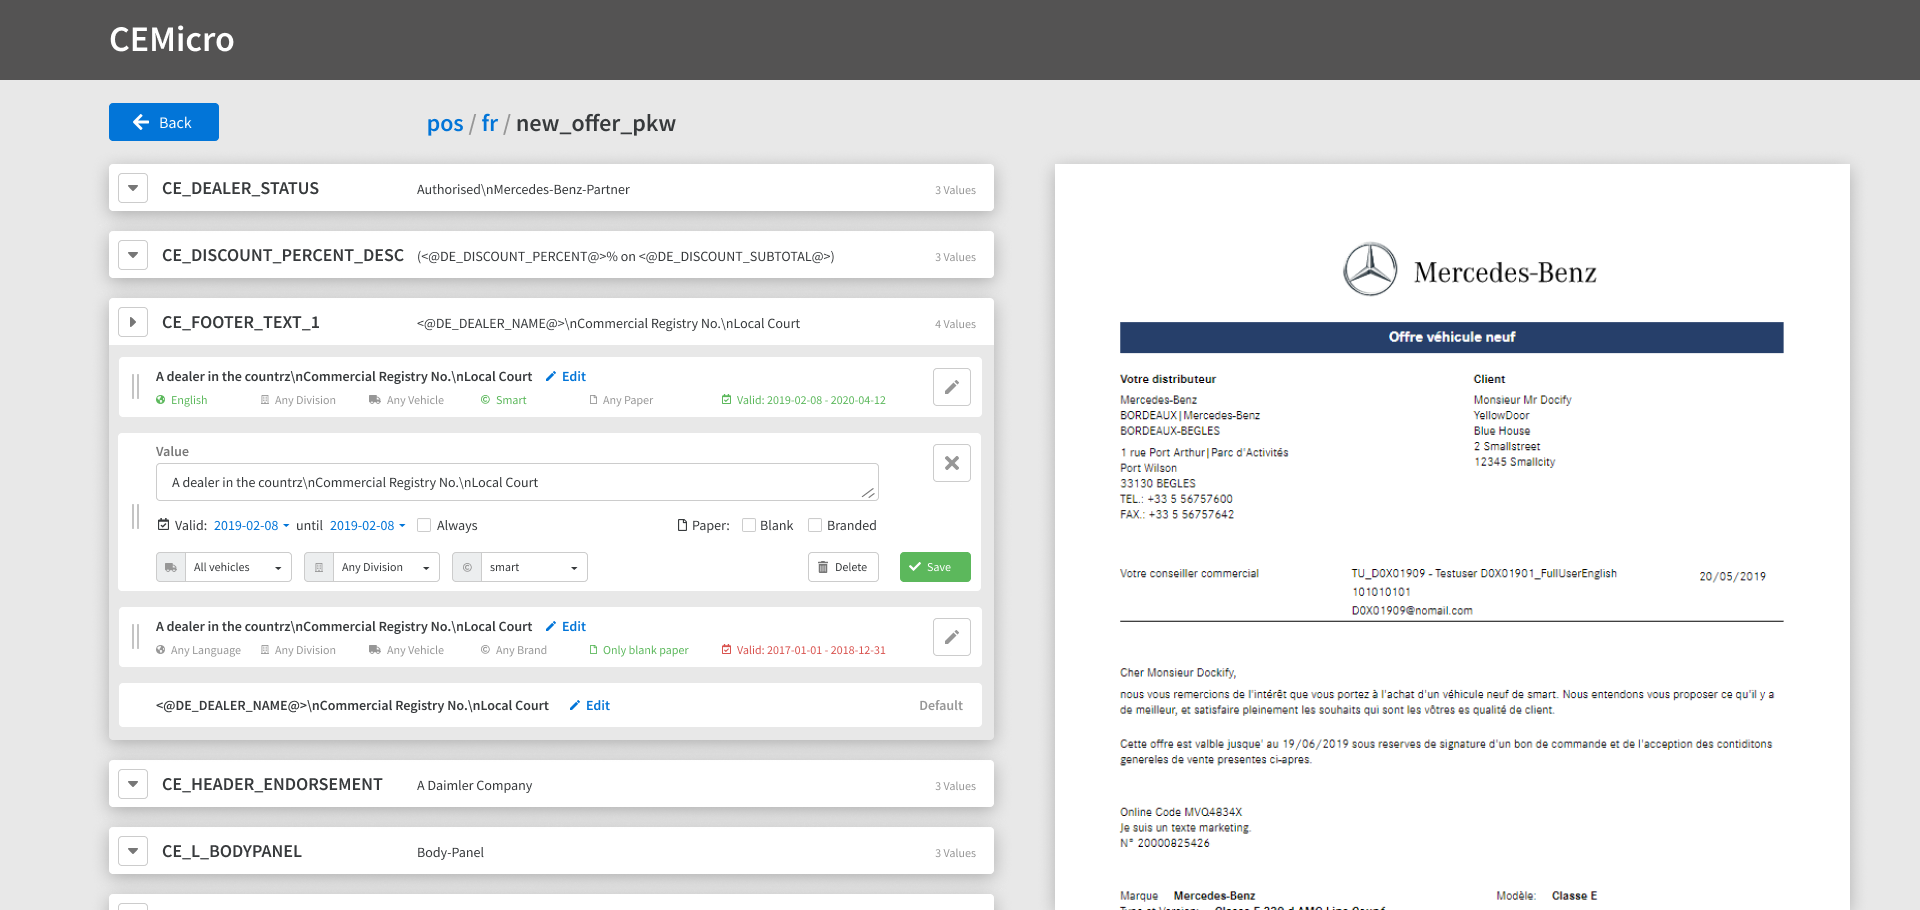
\includegraphics[width=\linewidth]{assets/cemicro-ui-mockup.png}
  \caption{User Interface mockup for CEMicro}
  \label{fig:mockup}
\end{figure}


